%%%%%%%%%%%%%%%%%%%%%%%%%%%%%%%%%%%%%%%%%
% Short Sectioned Assignment
% LaTeX Template
% Version 1.0 (5/5/12)
%
% This template has been downloaded from:
% http://www.LaTeXTemplates.com
%
% Original author:
% Frits Wenneker (http://www.howtotex.com)
%
% License:
% CC BY-NC-SA 3.0 (http://creativecommons.org/licenses/by-nc-sa/3.0/)
%
%%%%%%%%%%%%%%%%%%%%%%%%%%%%%%%%%%%%%%%%%

%----------------------------------------------------------------------------------------
%	PACKAGES AND OTHER DOCUMENT CONFIGURATIONS
%----------------------------------------------------------------------------------------

\documentclass[paper=a4, fontsize=11pt]{scrartcl} % A4 paper and 11pt font size

\usepackage[T1]{fontenc} % Use 8-bit encoding that has 256 glyphs
\usepackage{fourier} % Use the Adobe Utopia font for the document - comment this line to return to the LaTeX default
\usepackage[english]{babel} % English language/hyphenation
\usepackage{amsmath,amsfonts,amsthm} % Math packages

\usepackage{lipsum} % Used for inserting dummy 'Lorem ipsum' text into the template

\usepackage{sectsty} % Allows customizing section commands
\allsectionsfont{ \normalfont\scshape} % Make all sections centered, the default font and small caps

\usepackage{fancyhdr} % Custom headers and footers
\pagestyle{fancyplain} % Makes all pages in the document conform to the custom headers and footers
\fancyhead{} % No page header - if you want one, create it in the same way as the footers below
\fancyfoot[L]{} % Empty left footer
\fancyfoot[C]{} % Empty center footer
\fancyfoot[R]{\thepage} % Page numbering for right footer
\renewcommand{\headrulewidth}{0pt} % Remove header underlines
\renewcommand{\footrulewidth}{0pt} % Remove footer underlines
\setlength{\headheight}{13.6pt} % Customize the height of the header

\numberwithin{equation}{section} % Number equations within sections (i.e. 1.1, 1.2, 2.1, 2.2 instead of 1, 2, 3, 4)
\numberwithin{figure}{section} % Number figures within sections (i.e. 1.1, 1.2, 2.1, 2.2 instead of 1, 2, 3, 4)
\numberwithin{table}{subsection} % Number tables within sections (i.e. 1.1, 1.2, 2.1, 2.2 instead of 1, 2, 3, 4)

\setlength\parindent{0pt} % Removes all indentation from paragraphs - comment this line for an assignment with lots of text

\usepackage{graphicx}

\usepackage{geometry}
\geometry{left=2.5cm,right=2.5cm,top=2cm, bottom=3cm}

\usepackage{subfigure}
\usepackage{latexsym}

\usepackage{listings}
\usepackage{color}

\definecolor{codegreen}{rgb}{0,0.6,0}
\definecolor{codegray}{rgb}{0.5,0.5,0.5}
\definecolor{codepurple}{rgb}{0.58,0,0.82}
\definecolor{backcolour}{rgb}{0.95,0.95,0.92}

\lstdefinestyle{mystyle}{
	backgroundcolor=\color{backcolour},   
	commentstyle=\color{codegreen},
	keywordstyle=\color{magenta},
	numberstyle=\tiny\color{codegray},
	stringstyle=\color{codepurple},
	basicstyle=\footnotesize,
	breakatwhitespace=false,         
	breaklines=true,                 
	captionpos=b,                    
	keepspaces=true,                 
	numbers=left,                    
	numbersep=5pt,                  
	showspaces=false,                
	showstringspaces=false,
	showtabs=false,                  
	tabsize=2
}

\lstset{style=mystyle}

%----------------------------------------------------------------------------------------
%	TITLE SECTION
%----------------------------------------------------------------------------------------

\newcommand{\horrule}[1]{\rule{\linewidth}{#1}} % Create horizontal rule command with 1 argument of height
\title{CS767 Assignment 3}
\title{	
	\normalfont \normalsize 
	\textsc{University of Wisconsin-Madison, Computer Science Department} \\ [25pt] % Your university, school and/or department name(s)
	\horrule{0.5pt} \\[0.4cm] % Thin top horizontal rule
	\huge CS767 - Assignment 3 \\ % The assignment title
	\horrule{2pt} \\[0.5cm] % Thick bottom horizontal rule
}

\author{Zhicheng Gu \\ Email: zgu58@wisc.edu \\ Student ID: 9073696370} % Your name

\date{\normalsize\today} % Today's date or a custom date

\begin{document}
	
	\maketitle % Print the title
	
	%----------------------------------------------------------------------------------------
	%	PROBLEM 1
	%----------------------------------------------------------------------------------------
	% \renewcommand\thesection{\Alph{section}}
	\renewcommand\thesubsection{\arabic{subsection}}
	
	\section{Problem 1}
	
	I use Mutual information based registration to finish doMutInfoRegistration() method.
	calcMI() method is used to calculate the mutual information 
	of im2 and result of im1 after rotate a certain angle.
	In  method, fminsearch is used to find the min results.
	\\\\
	$fminsearch(@(k)calcMI(im1,im2,k),initialGuessAngle, options)$
	\\\\
	And the option is set to 100 to prevent the program from running too long.
	\\\\
	$options = optimset('MaxIter',100);$
	\\\\
	
	The results are shown in Figure 1.1 and Figure 1.2. 
	The best rotation angle for Figure 1 is -45.3442 and -24.9990 for Figure 2.
	
	
	
	\begin{figure}[!htbp]
		\centering
		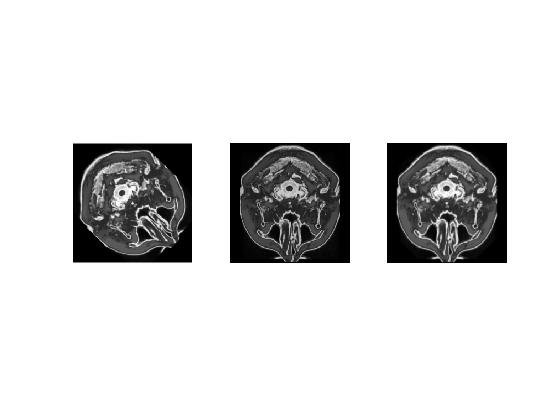
\includegraphics[width = 12cm]{p1.jpg}
		\caption{Result for Mutual information based registration}
	\end{figure}
	\begin{figure}[!htbp]
		\centering
		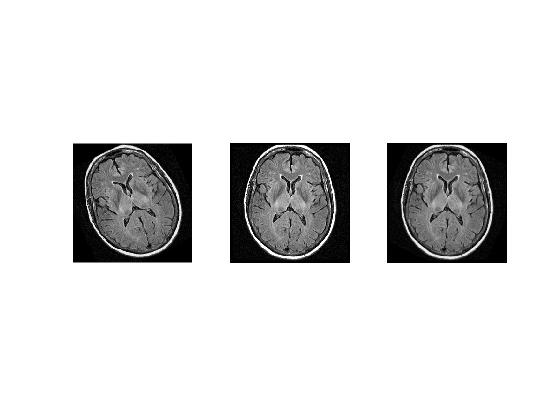
\includegraphics[width = 12cm]{p2.jpg}
		\caption{Result for Mutual information based registration}
	\end{figure}
	
	
	
	\newpage
	
	\section{Problem 2}
	
	Use normxcorr2() method to calculate the correlation of two images.
	The result for example is:
	
	xpeak = 134
	
	ypeak = 118
	
	scale = 0.5060
	
	(134, 118) is the bottom right corner of the small image.
	0.5060 is the scale of the small image.
	
	
	\section{Problem 3}
	
	I use a 15 * 15 non-overlapping regions to detect the optical flow.
	Use the best fit algorithm from the class to get the u and v for each region.
	
	The result for example image is shown in Firgure 3.1.
	
	\begin{figure}[!htbp]
		\centering
		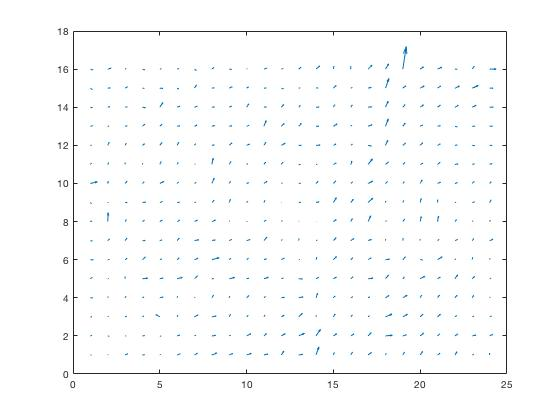
\includegraphics[width = 16cm]{p4.jpg}
		\caption{Optical flow}
	\end{figure}
	
	
	%----------------------------------------------------------------------------------------
	
\end{document}
